\chapter{La radioterapia adattiva. Implementazione iniziale e sviluppi futuri}
\minitoc
\textsf{In questo capitolo si passa ....}

\section{Origini e razionale della radioterapia adattiva}
Per radioterapia adattiva o \textit{adaptive radiation therapy} si intende una tecnica di erogazione della dose che di `adatta' ai possibili cambiamenti che si verificano durante il trattamento, rispetto alla situazione iniziale di pianificazione. I cambiamenti che si possono verificare durante un trattamento radiante possono essere di varia natura e riguardare sia l'interno del paziente (progressione/regressione del target, dimagrimento, diverso stato di riempimento degli organi cavi), sia il suo  posizionamento sul lettino di trattamento (incertezza di setup). Il metodo tradizionale di affrontare il problema dei cambiamenti rispetto alla situazione di pianificazione è esposto nei report della \textit{International Commission of Radiological Units} ICRU no.50 e no.62, ripreso anche nel recente report no.83 per le tecniche ad intensità modulata \cite{ICRU2010}. Esso consiste nell'espandere i target di un certo margine di sicurezza in modo da assicurare la loro corretta irradiazione anche in presenza di incertezze dovute al movimento degli organi interni e al posizionamento del paziente.
\begin{figure}
\centering
\includegraphics[width=.3\textwidth]{./cap3/ptv.png}
\includegraphics[width=.69\textwidth]{./cap3/adapt0.png}
\caption{Sinistra: definizioni ICRU dei volumi coinvolti nella pianificazione del trattamento radioterapico. Destra: Processo standard di pianificazione ed erogazione del piano del trattamento.}
\label{fig:adapt0}
\end{figure}

Nella Fig.\ref{fig:adapt0} sono riportate le definizioni dei volumi coinvolti nella pianificazione del trattamento radioterapico assieme ad uno schema del processo standard di pianificazione ed erogazione del piano del trattamento.\\
Il meccanismo che ha portato alla definizione dei vari volumi in radioterapia procede in vari step:
\begin{description}
\item[Gross Target Volume (GTV):] questo volume identifica il tumore a livello macroscopico (rivelabile attraverso strumenti ottici, imaging radiologico ed evenutale esame obiettivo del medico).

\item[Clinical Target Volume (CTV):] volume che comprende il GTV ed un margine attorno ad esso in cui vi è alta probabilità di presenza di malattia che ancora non si manifesta clinicamente (sub-clinica).

\item[Internal Target Volume (ITV):] volume che aggiunge al CTV un margine (detto \textit{internal margin o IM}) che serve a comprendere il possibile movimento del target per cause interne al paziente (e.g. respiro, stato di riempimento degli organi adiacenti, battito cardiaco\ldots).

\item[Planning Target Volume (PTV):] volume che aggiunge all'ITV un margine per comprendere l'incertezza dovuta al posizionamento del paziente rispetto alla posizione di pianificazione (\textit{setup margin o SM}).

\item[Treated Volume:] volume che riceve una dose maggiore del 98\% della dose di prescrizione.

\end{description}

Il metodo per calcolare i margini necessari alla definizione del PTV si basa su uno studio statistico in cui si effettua un analisi dei possibili errori di posizionamento del target rispetto alla posizione pianificata, distinguendoli in errori sistematici ed errori random. Una delle formule più note è dovuta a Marcel Van Herk \cite{ICRU62}:
\begin{equation}
PTV_{margin} = 2.5\Sigma + 0.7\sigma
\end{equation}
dove $\Sigma$ rappresenta l'errore sistematico ossia quell'errore che si ripete per tutto il ciclo di trattamento (es. paziente dimagrito rispetto alla pianficazione) mentre $\sigma$ è l'errore random (es. movimento d'organo).

In un approccio non adattivo i margini da dare al CTV per arrivare al PTV si trovano effettuando uno studio di coorte per un fissato sito di irradiazione. Nello studio si valutano gli errori sistematici e random su una popolazione di pazienti e si applica la formula di Van Herk secondo le direttive ICRU \cite{ICRU62}. La pianificazione viene quindi effettuata stabilendo delle condizioni di irradiazione del planning target volume (PTV)  che vengono ripetute per tutto il ciclo di trattamento (Fig.\ref{fig:adapt0}).\\
Questo tipo di approccio può tuttavia essere non è ottimale per lo specifico paziente come indicato schematicamente nella Fig.\ref{fig:margins}. In un approccio di \textit{adaptive radiotherapy} è invece possibile studiare il singolo caso ed adattare il trattamento allo specifico paziente.
\begin{figure}
\centering
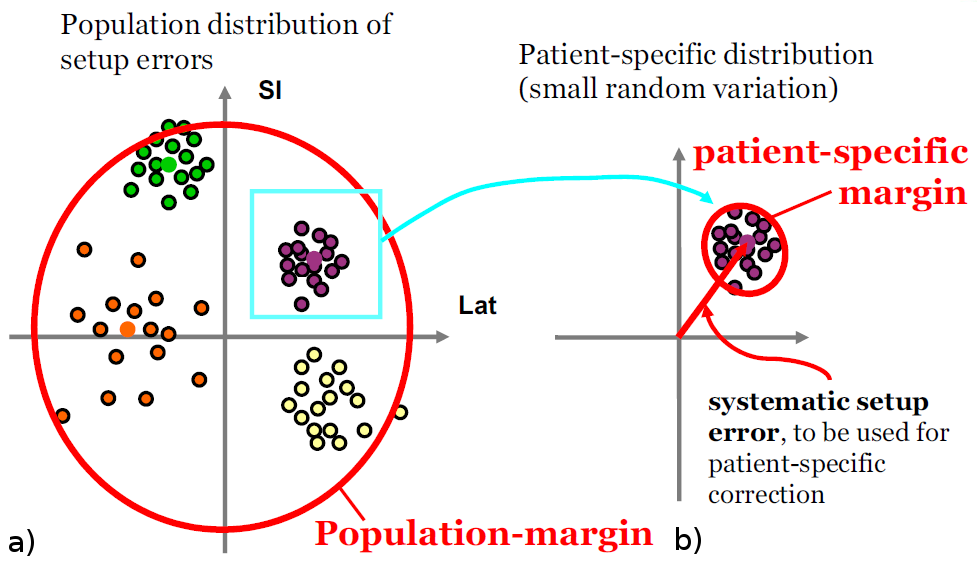
\includegraphics[width=.8\textwidth]{./cap3/margins.png}
\caption{La formula di Van Herk per ottenere il PTV utilizzando uno studio di coorte (sinistra) da luogo a margini che possono essere sovrabbondanti per il singolo paziente (destra).}
\label{fig:margins}
\end{figure}

Il termine \textit{adaptive radiotherapy} è stato introdotto per la prima volta  da Yan et al.\cite{Yan1996}. In questo lavoro veniva per la prima volta proposto un adattamento del piano di cura a seguito di rilevazioni effettuate nelle prime cinque sedute di trattamento con un dispositivo in grado di `fotografare' la posizione del paziente e di confrontarla rispetto alla posizione di pianficazione\footnote{Il dispositivo in oggetto è denominato \textit{portal imager} e consiste in un pannello elettronico montato sul LINAC ed è in grado di generare un'immagine utilizzando raggi di energia dell'ordine dei MeV uscenti dal LINAC allo stesso modo in cui vengono generate le radiografie classiche con i raggi di energia dell'ordine del keV.}. A seguito di queste rilevazioni Yan proponeva di stimare l'errore sistematico paziente-specifico calcolando la media delle deviazioni tra posizione pianificata e posizione di trattamento rilevate nelle prime cinque sedute e di adattare il piano spostando il centro di irradiazione di questa quantità.

\begin{figure}[!t]
\centering
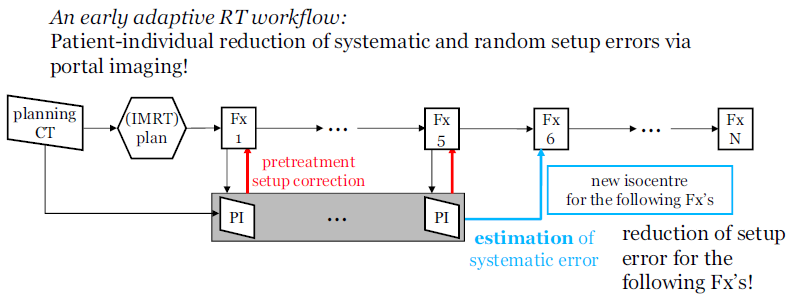
\includegraphics[width=\textwidth]{./cap3/adapt1.png}
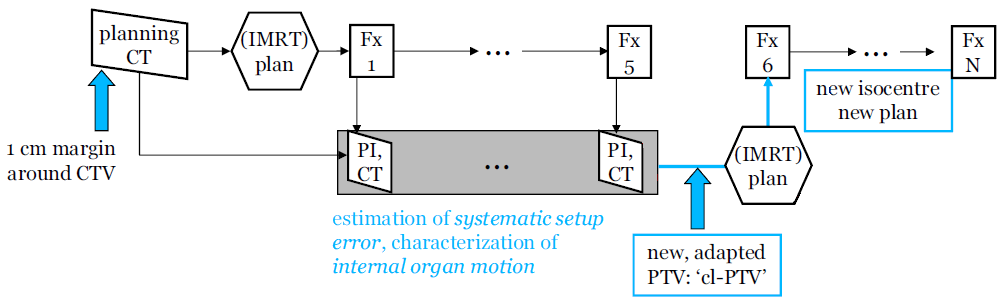
\includegraphics[width=\textwidth]{./cap3/adapt2.png}
\caption{Sopra: approccio di adaptive radiotherapy in cui viene unicamente modificato l'isocentro del piano a seguito di rilevazioni dell'errore di posizionamento del paziente tramite portal-imager (PI). Sotto: approccio di adaptive radiotherapy in cui alla modificazione dell'isocentro si aggiunge la modificazione dei margini attorno al CTV in base a rilevazioni di tomografia computerizzata (CT); in questo caso il piano di trattamento si adatta al nuovo PTV \textit{confidence-limit PTV o cl-PTV} stimato dopo le cinque sedute di controllo.}
\label{fig:adaptYAN}
\end{figure}

Pochi anni dopo sempre Yan et al.\cite{Yan2000} pubblicano un altro studio in cui aggiungono alla rilevazione tramite portal-imager anche un rilevazione di tomografia computerizzata del paziente per le prime cinque sedute in modo da osservare il problema del movimento d'organo oltre all'errore di setup. Questo permise agli autori di definire un PTV paziente-specifico che veniva calcolato con la procedura seguente:
\begin{itemize}
\item Si delineava il CTV sui cinque studi CT acquisite in sede delle prime cinque frazioni di trattamento.
\item Si uniscono i contorni dei cinque CTV con il CTV di pianficazione a costituire il cosiddetto \textit{CTV-hull}.
\item Si espande il \textit{CTV-hull} del margine corrispondente all'errore sistematico misurato tramite le cinque rilevazioni tramite portal-imager per formare il \textit{confidence-limit PTV o cl-PTV}. 
\end{itemize}
Entrambi gli approcci adaptive presentati in questa sezione sono raffigurati schematicamente nella Fig.\ref{fig:adaptYAN}.

\`E stato dimostrato che la riduzione del PTV e la conseguente ripianficazione possibile grazie all'applicazione di queste tecniche di adaptive radiotherapy ha portato ad un decremento significativo delle tossicità per gli organi sani, preservando il controllo della malattia \cite{Park2012}. Questo dato è facilmente comprensibile con il paradigma dell'arancia di Verellen \cite{Verellen2007} illustrato in Fig.\ref{fig:verellen}.
\begin{figure}[!t]
\centering
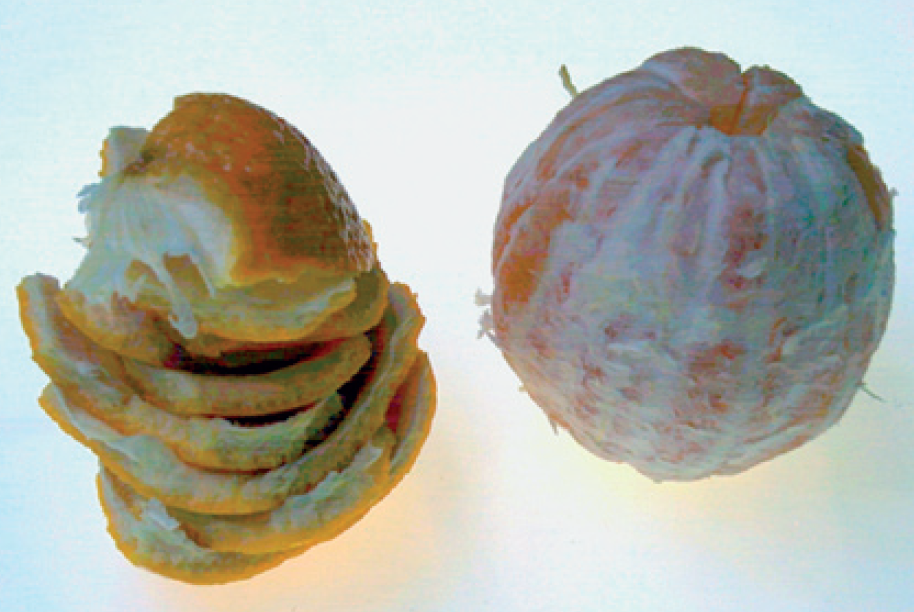
\includegraphics[width=.6\textwidth]{./cap3/Verellen.png}
\caption{Il paradigma dell'arancia di Verellen \cite{Verellen2007} per illustrare l'importanza della riduzione dei margini in radioterapia. In pratica il volume occupato dalla buccia di un arancia è comparabile con il volume dell'arancia stessa. La riduzione anche di pochi millimetri del PTV può comportare una riduzione del volume da irradiare considerevole che si traduce in un maggior risparmio dei tessuti sani.}
\label{fig:verellen}
\end{figure}



\section{Il concetto attuale di \textit{adaptive-radiotherapy} implementato in RayStation}
Il concetto di radioterapia adattiva ha subito negli anni vari aggiornamenti e revisioni ma solo negli ultimi anni è divenuto oggetto di grande interesse. Ciò è dovuto principalmente all'avvento  delle tecniche di imaging per il controllo volumetrico del posizionamento del paziente installate sui moderni LINAC\footnote{La tecnica più diffusa implementata nei moderni LINAC è denominata \textit{cone-beam-computed-tomography o CBCT}. Essa consiste in un sistema capace di ricostruire immagini tomografiche del paziente utilizzando un fascio conico di raggi X e di confrontarle con lo studio CT di pianificazione.}.

\begin{figure}[!t]
\centering
\centerline{
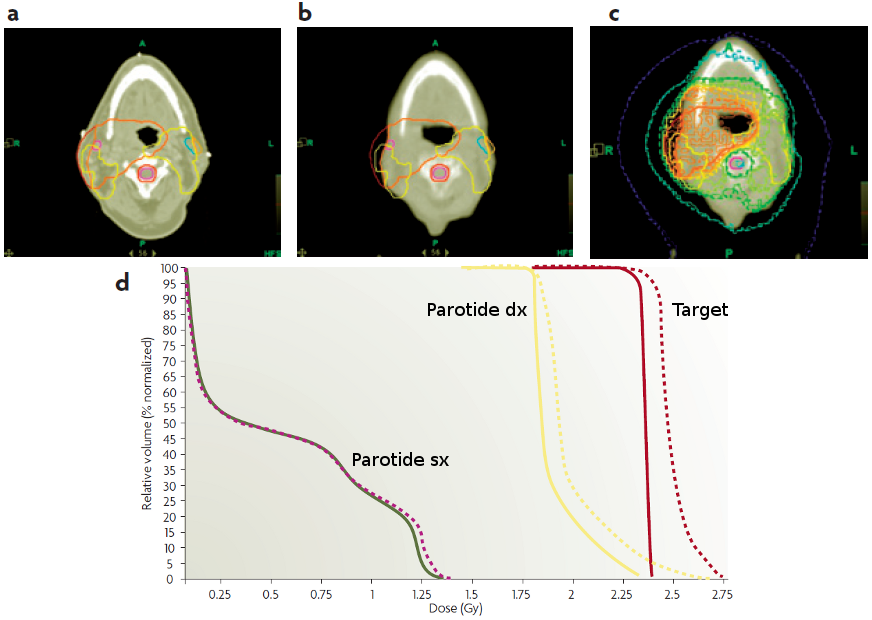
\includegraphics[width=1.2\textwidth]{./cap3/HN_DVH.png}}
\caption{(a) scansione CT del distretto testa-collo di un paziente con delineato in rosso il target e negli altri colori gli organi a rischio. (b) scansione CBCT di controllo a 2.5 settimane con evidente riduzione di volume del target. (c-d) confronto delle distribuzioni di dose di pianificazione (linea continua) e di valutazione (linea tratteggiata). L'istogramma (d) è detto \textit{istogramma dose-volume o DVH} e rappresenta quantitativamente come la distribuzione di dose copre i volumi delineati nello studio CT. \`E da notare come il cambiamento del paziente comporti una variazione della distribuzione di dose agli organi e al target.}
\label{fig:HN_DVH}
\end{figure}

 Nella Fig.\ref{fig:HN_DVH} è illustrato un tipico esempio di irradiazione del distretto testa-collo di largo interesse per la radioterapia adattiva per i grossi cambiamenti che avvengono in itinere nell'anatomia del paziente. A causa dei rapidi gradienti di dose realizzati con le tecniche ad intensità modulata, piccoli cambiamenti di anatomia del paziente possono avere un largo impatto sulla distribuzione di dose finale sia per il target che per gli organi a rischio (Fig.\ref{fig:HN_DVH}d). \\
 
Il TPS RayStation affronta il problema della radioterapia adattiva offrend una soluzione `all-in-one' che si articola in cinque principali step:
\begin{description}
\item[1) Acquisizione degli studi CBCT:] le CBCT acquisite dal sistema di imaging montato sul LINAC vengono spedite al TPS.
\item[2) Deformazione elastica:] viene effettuata una registrazione elastica tra la CT di pianificazione e le CBCT. Questa operazione consiste nel trovare il campo di deformazione geometrico che, se applicato alla CBCT di controllo,   trasforma quest'ultima nella CT di pianificazione. La trasformazione in oggetto è unicamente geometrica: vengono solo variate le coordinate dei pixel ma non il loro valore in scala di grigi.
\item[3) Calcolo della dose in CBCT:] il piano di trattamento viene trasferito alle CBCT e ricalcolato in modo da ottenere la distribuzione di dose relativa alle specifiche frazioni. 
\item[4) Deformazione delle dosi:] sulla base della registrazione deformabile geometrica viene deformata la distribuzione di dose calcolata in CBCT e riportata sulla CT di pianificazione. In questo modo si possono confrontare le distribuzioni di dose pianificata ed effettivamente erogata sulla CT di pianificazione.
\item[5) Adattamento del piano:] sulla base delle differenze tra le distribuzioni di dose pianificata ed erogata si decide o meno di effettuare una ripianificazione del trattamento.
\end{description}

Tutti questi passaggi (a parte il primo) presentano delle criticità che al giorno d'oggi non sono del tutto superate in maniera condivisa. In particolare, le questioni su cui vi è ancora un largo dibattito nella comunità scientifica possono essere riassunte nei punti seguenti:\\

\noindent\textbf{Deformazione elastica:}
\begin{itemize}
\item Quale accuratezza è raggiungibile?
\item Quale è il miglior modo di effettuare le deformazioni?
\end{itemize}
\textbf{Calcolo della dose in CBCT}
\begin{itemize}
\item Quanto è accurato il calcolo della dose in CBCT?
\item Calibrare o non calibrare la CBCT in termini di scala di grigi - densità?
\end{itemize}
\textbf{Deformazione delle dosi:}
\begin{itemize}
\item Quanto è giusto deformare le dosi applicando la trasformazione geometrica?
\end{itemize}
\textbf{Adattamento del piano:}
\begin{itemize}
\item Sulla base di quale metrica si può decidere la ripianificazione?
\item Qual è il momento migliore per la ripianificazione?
\item Che livello di verifica pre-trattamento è richiesto per il piano adattato?
\end{itemize}

La comunità scientifica non è ancora giunta ad una risposta precisa ed esaustiva per le domande sopra elencate per cui il commissioning del TPS dal punto di vista della radioterapia adattiva risulta tutt'ora (Febbraio 2016) in fase di ottimizzazione. In particolare, gli sforzi che si stanno compiendo in questo senso consistono nella partecipazione a due studi multicentrici nazionali orientati a chiarire gli aspetti più dibattuti ossia quelli riguardanti la deformazione elastica e l'adattamento del piano.

\subsection{Studio multicentrico per l'ottimizzazione del protocollo di deformazione elastica}
Il TPS RayStation implementa un algoritmo di deformazione elastica ibrido \cite{RaySearchLaboratories2014}. In un primo step il campo di deformazione viene calcolato considerando unicamente la differenza tra i livelli di grigio dello studio di riferimento e quello da deformare. In seconda battuta è possibile migliorare la deformazione `guindandola' con dei contorni geometrici (ROI di controllo).

Ciò si realizza matematicamente minimizzando un funzionale cha ha la forma seguente:
\begin{equation}
\label{eq:def}
\begin{split}
F =& \alpha \cdot (1- Correlation\, Coefficient) + \\
   & + \beta \cdot Regularization\,Term + \\
   & + \gamma \cdot ROI\,Penalty\,Term
\end{split}
\end{equation}
dove il \textit{Correlation coefficient} è un termine del tipo coefficiente di correlazione di Pearson e misura la correlazione tra i livelli di grigio delle due immagini (è uguale a 1 per immagini identiche). Il termine di regolarizzazione (\textit{Regularization Term}) aumenta all'aumentare dell'intensità della deformazione e serve a penalizzare soluzioni improbabili dal punto di vista fisico. Infine il \textit{ROI Penalty Term} è un termine che diminuisce quanto più le ROI di controllo tra le due immagini sono sovrapposte.

Nella corrente implementazione dell'algoritmo di deformazione in RayStation (v.4.7) i termini peso $\alpha$, $\beta$ e $\gamma$, il coefficiente di correlazione ed il termine di regolarizzazione sono tutti fissati dalla ditta. Quello che viene lasciato all'operatore è la scelta delle ROI di controllo ossia la forma dell'ultimo termine della Eq.\eqref{eq:def}.

Il razionale dello studio multicentrico cui si è presi parte consiste nell'investigare l'accuratezza di vari algoritmi di registrazione deformabile e di sviluppare le metodologie che portano alla migliore deformazione possibile. A questo proposito è stato riunito un gruppo di 13 istituzioni italiane (Gruppo YES) per un totale di 5 diverse soluzioni commerciali per la registrazione elastica, tra cui il TPS RayStation. Lo studio si articola in più fasi ed è tutt'ora (Febbraio 2016) in corso di svolgimento. Nell'ambito di questo lavoro di tesi discuteremo i risultati raggiunti nella fase riguardante i casi clinici.

Per la fase clinica dello studio YES sono stati reclutati 3 studi CT per i distretti pelvico, testa-collo e polmonare (Fig.\ref{fig:YES_sites}).
\begin{figure}
\centering
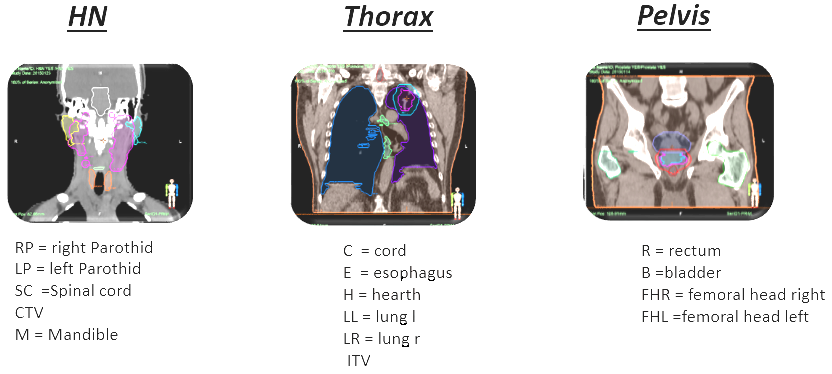
\includegraphics[width=\textwidth]{./cap3/YES_Sites.png}
\caption{Siti anatomici studiati nell'ambito del gruppo YES}
\label{fig:YES_sites}
\end{figure}
Per ogni distretto è stato creato un altro studio CT in cui è stata simulate tramite software (ImSimQA) una deformazione che tipicamente si realizza nella routine clinica:
\begin{description}
\item[Distretto pelvico:] riempimento vescicale minore rispetto alla CT di pianificazione.
\item[Distretto testa-collo:] riduzione di volume delle parotidi.
\item[Distretto polmonare:] riduzione di volume del tumore.
\end{description}
Ogni istituzione aveva il compito di ricavare in maniera inversa la deformazione simulata utilizzando gli strumenti in proprio possesso. Sulla base della deformazione ottenuta veniva richiesto di mappare delle regioni di interesse (ROI) dalla CT iniziale alla CT deformata. Le ROI mappate da ogni centro sono state poi confrontate con le ROI `gold' deformate secondo la deformazione simulata, nota solo al centro coordinatore.\\
L'indicatore utilizzato per confrontare le ROI mappate dai centri con le ROI `gold' è l'indice di conformità di Jaccard:
%\begin{equation}
%J(ROI_{A},ROI_{B{) = \frac{|ROI_{A} \cap ROI_{B}|}{|ROI_{A} \cup ROI_{B}|}
%\end{equation}
Questo indice è uguale a zero per ROI disgiunte mentre è uguale a uno per ROI esattamente sovrapposte.
I risultati raggiunti a livello multicentrico sono riassunti nella Fig.\ref{fig:YES_results} e possono essere riassunti principalmente nei seguenti punti:
\begin{itemize}
\item La differenza tra le performance globali dei vari centri non è risultata statisticamente significativa tranne che per un centro (Fig.\ref{fig:YES_results}a). 
\item La deformazione è risultata statisticamente più accurata  nel caso torace piuttosto che i casi pelvici e testa-collo (Fig.\ref{fig:YES_results}b).
\end{itemize}
\begin{figure}
\centering
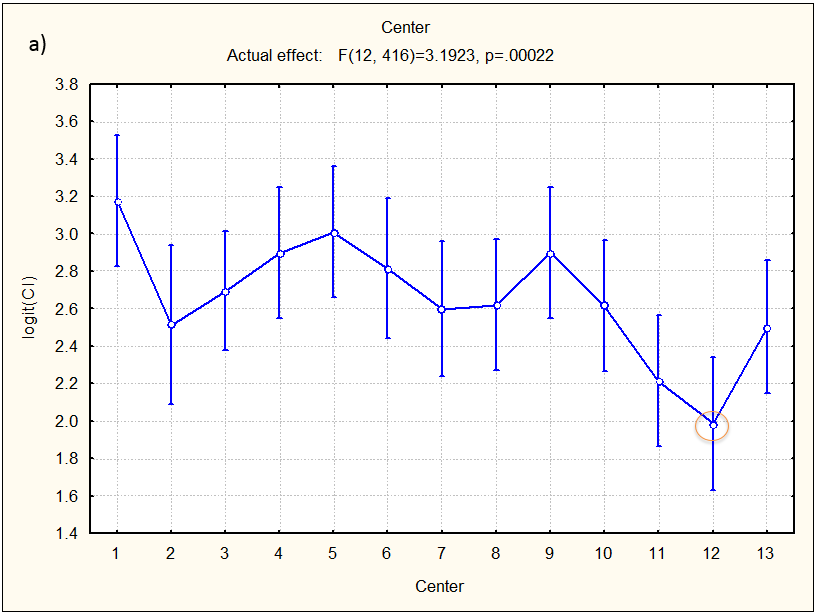
\includegraphics[width=.49\textwidth]{./cap3/YES_results_a.png}
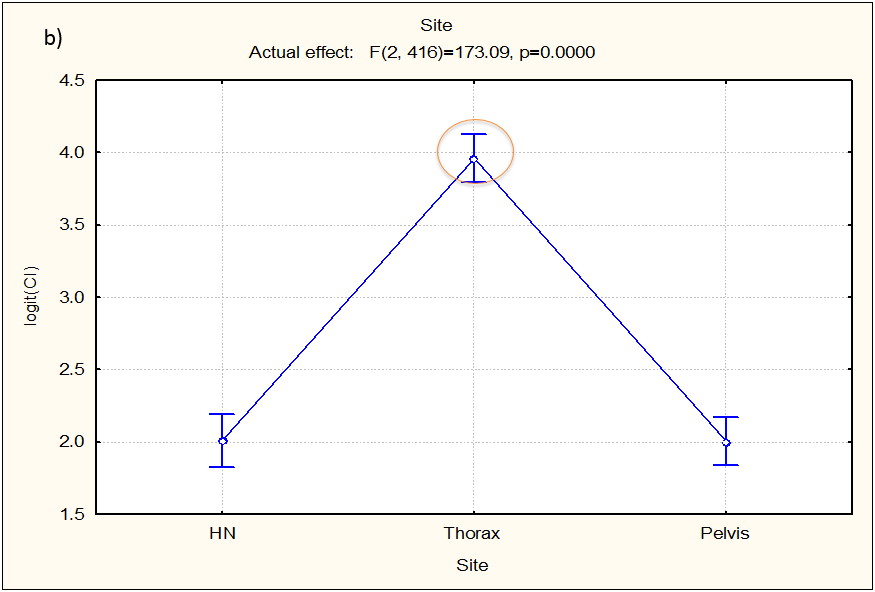
\includegraphics[width=.49\textwidth]{./cap3/YES_results_b.png}
\caption{(a) risultati del confronto per quanto riguarda l'accuratezza globale delle deformazioni effettuate dai singoli centri. (b) risultati dell'accuratezza raggiunta considerando tutti i centri a seconda del sito di interesse. I valori statisticamente differenti dal campione sono cerchiati in rosso. Il test statistico utilizzato è del tipo ANOVA (\textit{ANalysis Of VAriances}).}
\label{fig:YES_results}
\end{figure}
Dal primo risultato si può evincere che le soluzioni commerciali esistenti portano a soluzioni di precisione comparabile pur implementando algoritmi differenti tra loro. Le performance centro statisticamente differente sono imputabili ad differente livello di training degli operatori coinvolti.

Il secondo risultato è spiegabile con la peculiarità del sito toracico (tumore polmonare) rispetto ai siti testa-collo e pelvico. In questi ultimi, molti dei tessuti coinvolti risultano essere differenti di pochi livelli nella scala di grigi (basso contrasto) per cui è necessario guidare la deformazione con varie ROI di controllo (il coefficiente di correlazione dei grigi non è sufficiente ad ottenere una deformazione accurata). Diversa è la situazione per il caso toracico in cui il tessuto tumorale all'interno del polmone risulta essere ad alto contrasto con il tessuto circostante per cui la deformazione risulta semplice da trovare da parte dell'algoritmo, senza l'ausilio di particolari `aiuti'.

Continuare qui parlando dei risultati ottenuti a livello locale e della bozza dei protocolli di deformazione


\subsection{Studio multicentrico per predire la necessità di adattare il piano}
Continua qui prendi i risultati dell'AIFM etc etc
sottosezione adaptive (GUIDI) con risultati preliminari tipo quella roba delle parotidi etc etc e siamo quasi quasi per finire :OOO









